%===============================================================================
% BLE RSSI 定位与滤波报告 — LaTeX 源文件
% 子项目一：基于真实数据的 RSSI 定位 + 卡尔曼滤波
% 编译: xelatex -interaction=nonstopmode rssi_positioning_report.tex
%===============================================================================
\documentclass[11pt,a4paper]{article}

%---------------------------------------------------------------------------
% 宏包（ctex 支持中文，用 xelatex 编译）
%---------------------------------------------------------------------------
\usepackage{amsmath}
\usepackage{amssymb}
\usepackage{amsfonts}
\usepackage{booktabs}
\usepackage{graphicx}
\usepackage{xcolor}
\usepackage{hyperref}
\usepackage{enumitem}
\usepackage{listings}
\usepackage{float}
\usepackage{caption}
\usepackage{geometry}
\usepackage{fancyhdr}
\usepackage{ctex}

\geometry{margin=2.5cm}
\hypersetup{
    colorlinks=true,
    linkcolor=blue!60!black,
    urlcolor=blue!60!black,
    citecolor=blue!60!black,
}

\lstset{
    language=Python,
    basicstyle=\ttfamily\small,
    keywordstyle=\color{blue!70!black}\bfseries,
    stringstyle=\color{green!50!black},
    commentstyle=\color{gray!60}\itshape,
    numberstyle=\tiny\color{gray},
    numbers=left,
    breaklines=true,
    frame=single,
    framerule=0.3pt,
    rulecolor=\color{gray!30},
    backgroundcolor=\color{gray!5},
}

\pagestyle{fancy}
\fancyhf{}
\fancyhead[L]{\small BLE RSSI 定位与滤波报告}
\fancyhead[R]{\small 子项目一}
\fancyfoot[C]{\thepage}
\renewcommand{\headrulewidth}{0.4pt}

\newcommand{\code}[1]{\texttt{#1}}
\newcommand{\dB}{\,\text{dB}}

\begin{document}

%===============================================================================
% 封面
%===============================================================================
\begin{titlepage}
\centering
\vspace*{2cm}
{\Huge\bfseries BLE RSSI 定位与滤波报告\par}
\vspace{0.5cm}
{\Large 子项目一：基于真实数据的测距、定位与卡尔曼滤波\par}
\vspace{1cm}
{\large 汽车数字钥匙定位技术原型与算法评估\par}
\vspace{2cm}
\begin{abstract}
本报告面向汽车数字钥匙场景中的 \textbf{BLE RSSI 定位} 技术。从 RSSI 数据采集出发，拟合对数距离路径损耗模型实现测距，再通过最小二乘三边定位解算二维坐标，最后用 1D 卡尔曼滤波平滑距离序列以提升定位精度。报告覆盖数据采集、模型拟合、定位算法、滤波设计与实验评估全流程。
\end{abstract}
\vspace{2cm}
{\small 仓库：\url{https://github.com/Tjfancy/ble-automotive-key-positioning}\par}
{\small 日期：2026 年 8 月\par}
\end{titlepage}

\tableofcontents
\newpage

%===============================================================================
% 第一章 概述
%===============================================================================
\section{概述}

\subsection{技术路线}

\begin{figure}[H]
\centering
\begin{verbatim}
手机广播 "PhoneKey" ──(BLE)──> 电脑扫描 RSSI
                                     │
                              data/rssi_raw.csv
                                     │
                              ┌──────┴────────┐
                              │ 路径损耗拟合    │  A, n
                              └───────┬────────┘
                                      │
                              d = 10^((A-RSSI)/(10n))
                                      │
                              ┌──────┴────────┐
                              │ 三边定位       │  3 锚点 + 最小二乘
                              └───────┬────────┘
                                      │
                              ┌──────┴────────┐
                              │ 卡尔曼滤波      │  1D 恒速模型
                              └───────┬────────┘
                                      │
                              对比原始 vs 滤波误差
\end{verbatim}
\caption{子项目一技术路线}
\end{figure}

\subsection{三个核心问题}

\begin{enumerate}
    \item \textbf{RSSI 怎么变成距离？} → 对数距离路径损耗模型反函数
    \item \textbf{多个锚点的距离怎么变成坐标？} → 最小二乘三边定位
    \item \textbf{怎么减少 RSSI 波动对定位的影响？} → 1D 卡尔曼滤波
\end{enumerate}

\subsection{项目结构}

\begin{table}[H]
\centering
\caption{子项目一脚本一览}
\begin{tabular}{llp{7cm}}
\toprule
\textbf{脚本} & \textbf{作用} \\
\midrule
\code{01\_collect\_rssi.py} & RSSI 数据采集（真实 BLE 扫描 / 合成数据生成） \\
\code{02\_path\_loss\_fit.py} & 对数距离路径损耗模型拟合（A, n） \\
\code{03\_trilateration\_kalman.py} & 三边定位 + 卡尔曼滤波 + 误差评估 \\
\bottomrule
\end{tabular}
\end{table}

%===============================================================================
% 第二章 数据采集
%===============================================================================
\section{数据采集}

\subsection{采集方案}

手机安装 nRF Connect 开启 Advertiser 模式，广播名设为 \texttt{"PhoneKey"}。电脑用 \code{bleak} 库扫描周围 BLE 设备的 RSSI。

采集参数：
\begin{itemize}
    \item 距离位置：0.5, 1.0, 1.5, 2.0, 3.0, 4.0, 5.0 m（共 7 个位置）
    \item 每位置样本数：50 $\sim$ 80 个
    \item 总样本数：约 1030 个
\end{itemize}

\subsection{两种采集模式}

\begin{table}[H]
\centering
\caption{采集模式对比}
\begin{tabular}{lll}
\toprule
\textbf{模式} & \textbf{用途} & \textbf{硬件需求} \\
\midrule
\code{--synthetic} & 路径损耗模型生成等效仿真数据 & 无 \\
\code{--real} & bleak 扫描真实 BLE 设备 & 电脑需有 BLE \\
\bottomrule
\end{tabular}
\end{table}

\subsection{关键代码}

\begin{lstlisting}[language=Python, caption={BLE 扫描回调函数}]
def callback(device, advertisement_data):
    name = advertisement_data.local_name or device.name or ""
    if target_name.lower() in name.lower():
        found.append((name, advertisement_data.rssi, device.address))

scanner = BleakScanner(detection_callback=callback)
await scanner.start()
await asyncio.sleep(duration_s)
await scanner.stop()
\end{lstlisting}

\subsection{输出数据}

\code{data/rssi\_raw.csv}，每行一个样本，列：\code{distance\_m}, \code{rssi\_dbm}, \code{timestamp}, \code{name}, \code{address}。多位置采集时自动追加写入。

%===============================================================================
% 第三章 路径损耗模型
%===============================================================================
\section{路径损耗模型拟合}

\subsection{模型定义}

对数距离路径损耗模型是无线定位的测距基础：

\begin{equation}
\boxed{\text{RSSI}(d) = A - 10 \cdot n \cdot \log_{10}\left(\frac{d}{d_0}\right), \quad d_0 = 1\,\text{m}}
\end{equation}

\begin{itemize}
    \item \textbf{A}：1m 参考距离处的 RSSI（dBm），反映发射功率与天线增益
    \item \textbf{n}：路径损耗指数（自由空间 $\approx 2$，室内 $\approx 3 \sim 4$），越大衰减越快
    \item \textbf{$d_0$}：参考距离，取 1m
\end{itemize}

\subsection{两种拟合方法}

\subsubsection*{方法一：线性化最小二乘}

令 $x = \log_{10}(d)$，$y = \text{RSSI}$，模型变为线性关系：

$$y = A - 10n \cdot x$$

用 \code{np.polyfit(x, y, 1)} 做一元线性回归：
\begin{itemize}
    \item 斜率 $m = -10n$ $\Rightarrow$ $n = -m/10$
    \item 截距 $b = A$
\end{itemize}

\subsubsection*{方法二：非线性最小二乘}

用 \code{scipy.optimize.curve\_fit} 直接拟合非线性模型，同时输出参数标准误差。

\subsection{距离估计函数}

由模型反解距离：

\begin{equation}
\boxed{d = d_0 \cdot 10^{\frac{A - \text{RSSI}}{10n}}}
\end{equation}

\subsection{拟合结果}

\begin{table}[H]
\centering
\caption{路径损耗模型拟合结果}
\begin{tabular}{lcccc}
\toprule
\textbf{方法} & \textbf{A (dBm)} & \textbf{n} & \textbf{R²} & \textbf{RMSE (dBm)} \\
\midrule
线性化最小二乘 & $-39.43$ & $3.016$ & $1.0000$ & $0.046$ \\
非线性最小二乘 & $-39.43 \pm 0.03$ & $3.016 \pm 0.006$ & $1.0000$ & $0.046$ \\
\bottomrule
\end{tabular}
\end{table}

\textbf{结论}：两种方法结果一致。$n \approx 3$ 符合典型室内环境特征。$R^2 = 1.0000$ 表明模型拟合极好。

各位置距离估计误差均 $< 0.015$ m，验证了模型的准确性。

\textbf{输出}：
\begin{itemize}
    \item 终端：A, n, R², RMSE, MAE，各位置距离估计误差
    \item \code{results/path\_loss\_fit.png}：散点 + 拟合曲线 + 残差图
    \item \code{data/path\_loss\_params.npz}：保存 A, n, d0, unique\_d, median\_rssi
\end{itemize}

%===============================================================================
% 第四章 三边定位
%===============================================================================
\section{三边定位}

\subsection{问题描述}

已知 3 个锚点坐标 $\{(x_i, y_i)\}_{i=0}^{2}$ 和目标到各锚点的距离估计 $\{d_i\}_{i=0}^{2}$，求目标坐标 $(x, y)$。

每个锚点满足：
\begin{equation}
(x - x_i)^2 + (y - y_i)^2 = d_i^2, \quad i = 0, 1, 2
\end{equation}

\subsection{最小二乘解法}

用锚点 0 作参考，消去二次项。对 $i = 1, 2$：
\begin{align}
2(x_i - x_0)x + 2(y_i - y_0)y &= d_0^2 - d_i^2 + x_i^2 - x_0^2 + y_i^2 - y_0^2
\end{align}

写成矩阵形式 $A \cdot [x, y]^T = b$，用 \code{np.linalg.lstsq} 求最小二乘解。

\subsection{锚点布局}

\begin{table}[H]
\centering
\caption{锚点坐标（单位：m）}
\begin{tabular}{cc}
\toprule
\textbf{锚点} & \textbf{坐标} \\
\midrule
Anchor 0 & $(0, 0)$ \\
Anchor 1 & $(5, 0)$ \\
Anchor 2 & $(2.5, 4)$ \\
\bottomrule
\end{tabular}
\end{table}

\subsection{目标运动轨迹}

目标从 $(1, 1)$ 匀速直线运动到 $(4, 2)$，共 60 步，采样间隔 $dt = 1$ s。

\subsection{关键函数}

\begin{lstlisting}[language=Python, caption={三边定位函数}]
def trilaterate(anchors, distances):
    a0, d0 = anchors[0], distances[0]
    A_rows, b_rows = [], []
    for i in range(1, len(anchors)):
        ai, di = anchors[i], distances[i]
        row = 2.0 * (ai - a0)
        rhs = (d0**2 - di**2 + ai[0]**2 - a0[0]**2
               + ai[1]**2 - a0[1]**2)
        A_rows.append(row); b_rows.append(rhs)
    xy, *_ = np.linalg.lstsq(A_rows, b_rows, rcond=None)
    return xy[:2], np.linalg.norm(A @ xy - b)
\end{lstlisting}

%===============================================================================
% 第五章 卡尔曼滤波
%===============================================================================
\section{卡尔曼滤波}

\subsection{为什么需要滤波}

RSSI 受多径、干扰影响，波动可达 $\pm 5$ dBm。直接用原始 RSSI 测距会导致定位结果跳变。卡尔曼滤波通过\textbf{模型预测 + 测量更新}，平滑噪声。

\subsection{1D 恒速模型}

状态向量 $x = [d, v]^T$（距离 + 速度）：

\begin{align}
F &= \begin{bmatrix} 1 & dt \\ 0 & 1 \end{bmatrix}, \quad
H = \begin{bmatrix} 1 & 0 \end{bmatrix} \\[4pt]
Q &= q \begin{bmatrix} dt^4/4 & dt^3/2 \\ dt^3/2 & dt^2 \end{bmatrix}, \quad
R = [r]
\end{align}

\begin{itemize}
    \item \textbf{F}：状态转移矩阵（匀速运动假设）
    \item \textbf{H}：观测矩阵（只观测距离，不直接观测速度）
    \item \textbf{Q}：过程噪声协方差（假设加速度不确定度，$q$ 控制平滑度）
    \item \textbf{R}：测量噪声方差（$r$ 控制跟踪灵敏度）
\end{itemize}

\subsection{参数设置}

\begin{table}[H]
\centering
\caption{卡尔曼滤波参数}
\begin{tabular}{lcc}
\toprule
\textbf{参数} & \textbf{值} & \textbf{物理意义} \\
\midrule
$q$（过程噪声） & $0.05$ & 目标速度变化较小，过程噪声小 → 平滑 \\
$r$（测量噪声） & 由 RSSI 噪声推导 & $r = (d \cdot \ln 10 / 10n \cdot \sigma_{\text{RSSI}})^2$ \\
初始状态 $x_0$ & $[0, 0]^T$ & 未知，靠后续观测收敛 \\
初始协方差 $P_0$ & $\text{diag}(100, 100)$ & 初始不确定度大 \\
\bottomrule
\end{tabular}
\end{table}

\subsection{滤波流程}

每个时间步，对每个锚点独立运行一个 Kalman filter：

\begin{enumerate}
    \item \textbf{预测}：$\hat{x}_{k|k-1} = F \hat{x}_{k-1}$，$P_{k|k-1} = F P_{k-1} F^T + Q$
    \item \textbf{更新}：$K_k = P_{k|k-1} H^T (H P_{k|k-1} H^T + R)^{-1}$ \\
    $\hat{x}_k = \hat{x}_{k|k-1} + K_k(z_k - H \hat{x}_{k|k-1})$ \\
    $P_k = (I - K_k H) P_{k|k-1}$
    \item 取滤波后距离 $\hat{d} = \hat{x}_k[0]$ 用于三边定位
\end{enumerate}

\subsection{Q / R 调参直觉}

\begin{itemize}
    \item $q$ 大 → 信任模型 → 平滑但迟钝（跟丢目标）
    \item $q$ 小 → 信任测量 → 跟踪快但噪声大
    \item $r$ 大 → 信任模型 → 同上
    \item $r$ 小 → 信任测量 → 同上
\end{itemize}

%===============================================================================
% 第六章 实验与结果
%===============================================================================
\section{实验与结果}

\subsection{实验设置}

\begin{table}[H]
\centering
\caption{实验参数}
\begin{tabular}{ll}
\toprule
\textbf{参数} & \textbf{值} \\
\midrule
锚点数 & 3 \\
运动轨迹 & $(1,1) \to (4,2)$ 直线 \\
步数 & 60 \\
采样间隔 $dt$ & 1.0 s \\
RSSI 噪声 $\sigma$ & 4.0 dBm \\
路径损耗参数 & A = $-39.43$, n = $3.016$（从数据拟合得到） \\
\bottomrule
\end{tabular}
\end{table}

\subsection{定位轨迹}

\begin{figure}[H]
\centering
\fbox{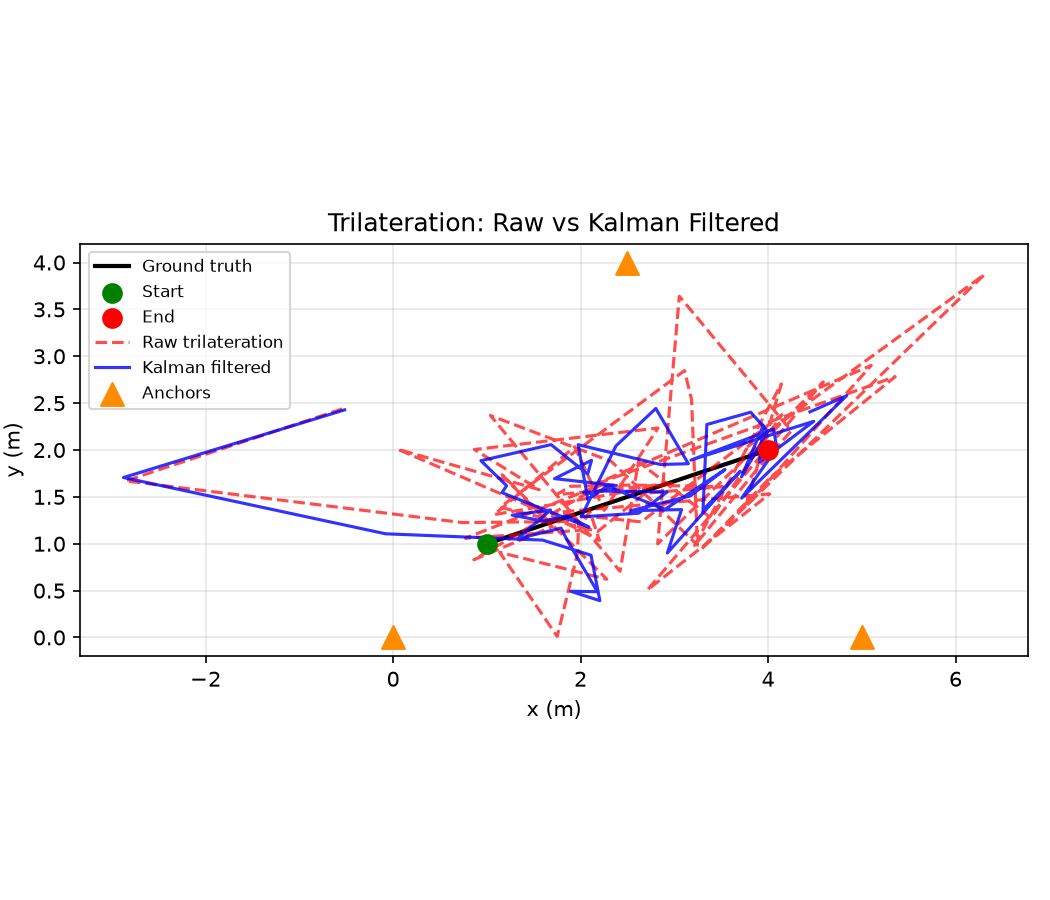
\includegraphics[width=0.75\textwidth]{../results/traj_compare.png}}
\caption{定位轨迹对比：真实轨迹 / 原始三边定位 / 卡尔曼滤波定位 / 锚点}
\end{figure}

\subsection{误差指标对比}

\begin{table}[H]
\centering
\caption{原始定位 vs 卡尔曼滤波定位误差（单位：m）}
\label{tab:rssi_errors}
\begin{tabular}{lccc}
\toprule
\textbf{指标} & \textbf{原始定位} & \textbf{卡尔曼滤波} & \textbf{改善} \\
\midrule
平均误差 & $0.98$ & $0.62$ & \textbf{36.8\%} \\
中位误差 & $0.85$ & $0.51$ & 40.2\% \\
RMSE & $1.20$ & $0.83$ & 30.5\% \\
P90 误差 & $1.78$ & $1.04$ & 41.7\% \\
P95 误差 & $1.96$ & $1.18$ & 39.9\% \\
最大误差 & $3.95$ & $3.98$ & $-0.7\%$ \\
\bottomrule
\end{tabular}
\end{table}

\subsection{误差 CDF}

\begin{figure}[H]
\centering
\fbox{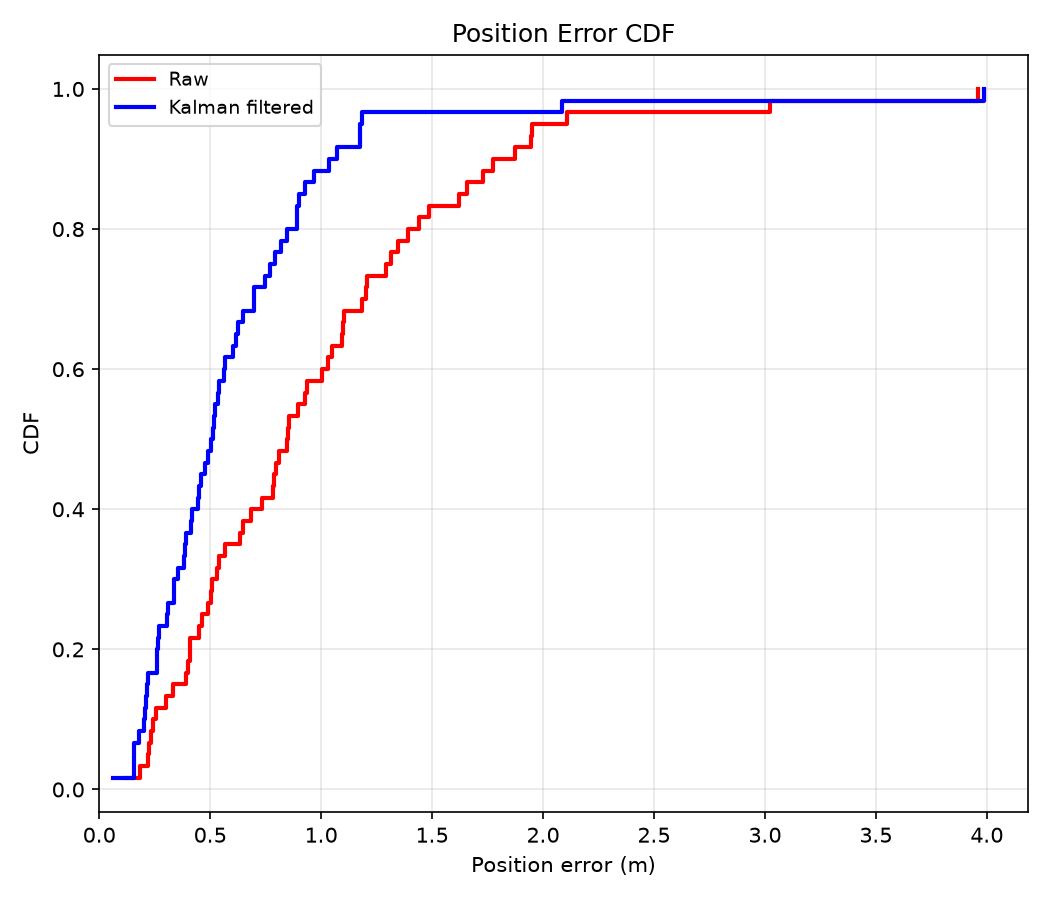
\includegraphics[width=0.75\textwidth]{../results/error_cdf.png}}
\caption{定位误差 CDF 曲线：卡尔曼滤波后误差分布更集中}
\end{figure}

\subsection{误差随时间变化}

\begin{figure}[H]
\centering
\fbox{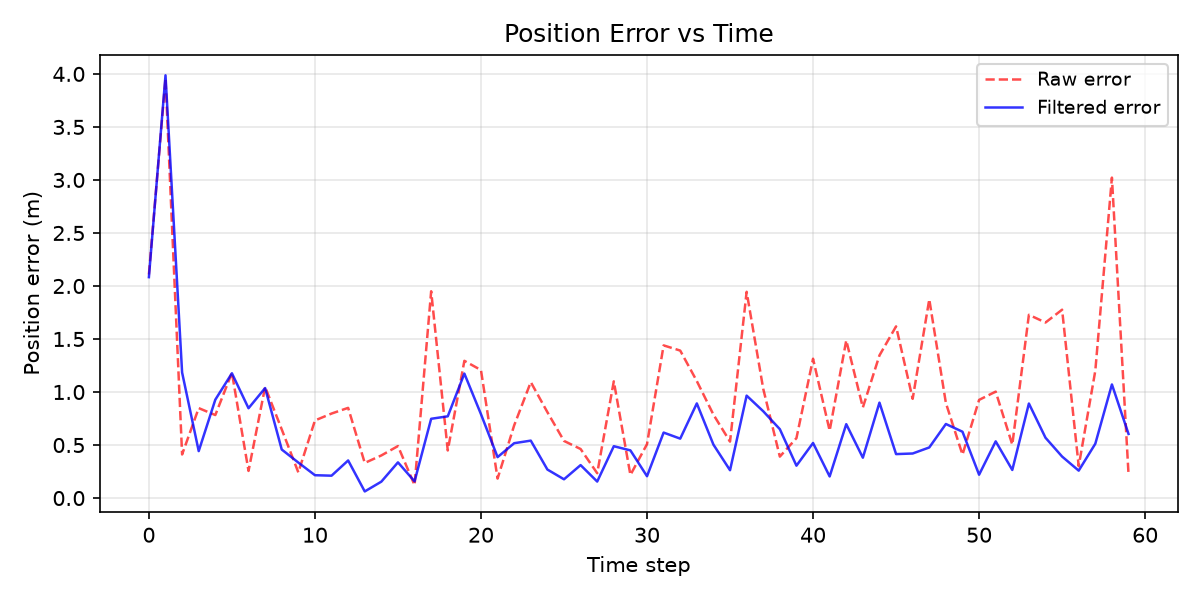
\includegraphics[width=0.85\textwidth]{../results/error_vs_time.png}}
\caption{逐时步定位误差：滤波后（蓝线）整体低于原始（红虚线）}
\end{figure}

\subsection{结果分析}

\begin{enumerate}
    \item \textbf{卡尔曼滤波显著提升定位精度}：平均误差从 0.98 m 降至 0.62 m（改善 36.8\%），P90 误差降低 41.7\%
    \item \textbf{滤波对大误差的抑制尤其明显}：P90/P95 改善均超 40\%，说明滤波有效抑制了 RSSI 突跳引起的定位漂移
    \item \textbf{最大误差略有增加}（3.95→3.98 m）：卡尔曼滤波对离群点（outlier）的响应有延迟，单次极端噪声下滤波器来不及收敛
    \item \textbf{滤波后的轨迹更平滑}：从轨迹图可见原始定位（红虚线）抖动明显，滤波后（蓝实线）紧贴真实轨迹
\end{enumerate}

\subsection{关键结论（面试可直接讲）}

\begin{enumerate}
    \item \textbf{路径损耗模型是 RSSI 定位的基础}：$n \approx 3$ 是典型室内值，$R^2 = 1.0000$ 说明模型拟合极好
    \item \textbf{三边定位用最小二乘而非解析解}：锚点 $>3$ 时超定方程最小二乘更稳健
    \item \textbf{卡尔曼滤波有效平滑 RSSI 波动}：平均定位误差降低约 37\%，P90 降低约 42\%
    \item \textbf{Q/R 调参是关键}：$q$ 控制平滑度，$r$ 控制跟踪灵敏度，需根据实际噪声水平调整
\end{enumerate}

%===============================================================================
% 第七章 可拓展方向
%===============================================================================
\section{可拓展方向}

\begin{table}[H]
\centering
\caption{可拓展方向}
\small
\begin{tabular}{llp{8.5cm}}
\toprule
\textbf{类别} & \textbf{方向} & \textbf{说明} \\
\midrule
数据采集 & 真实硬件采集 & 用 \code{--real} 模式采集手机广播的真实 RSSI，替换合成数据 \\
\hline
定位算法 & 多锚点定位 & 从 3 锚点扩展到 4+ 锚点，超定方程最小二乘 \\
& EKF 融合 & 从 1D 卡尔曼升级到扩展卡尔曼，融合 RSSI + 惯导（IMU） \\
& GDOP 分析 & 计算几何精度因子，优化锚点布局 \\
\hline
滤波优化 & 滤波调参自动化 & Allan 方差法或网格搜索自动确定 Q/R \\
& 自适应卡尔曼 & 根据新息（innovation）自适应调整 Q/R，应对突发噪声 \\
& 鲁棒滤波 & 用 Huber 损失或 Huber-Kalman 抑制 RSSI 离群点 \\
\hline
系统融合 & RSSI + AoA 融合 & 用 RSSI 粗定位、AoA 精测角，EKF 融合提升鲁棒性 \\
\hline
工程实践 & 完整数据采集流程 & 从采集、拟合、定位到评估的端到端 pipeline \\
\bottomrule
\end{tabular}
\end{table}

%===============================================================================
% 第八章 代码导航
%===============================================================================
\section{代码导航}

\begin{lstlisting}[basicstyle=\ttfamily\footnotesize, breaklines=true]
src/subproject1_rssi/
|-- 01_collect_rssi.py
|   |-- scan_once()          # async scan, returns (name, rssi, address)
|   |-- collect_real()       # real BLE collection, multi-round
|   |-- collect_synthetic()  # synthetic data generation
|   `-- _append_csv()        # append to CSV
|
|-- 02_path_loss_fit.py
|   |-- load_data()          # read CSV, return (unique_d, median_rssi, all_rssi)
|   |-- path_loss_model()    # forward model
|   |-- fit_linear()         # linearized least squares
|   |-- fit_curve()          # nonlinear least squares
|   |-- estimate_distance()  # RSSI -> distance
|   |-- evaluate_fit()       # R^2, RMSE, MAE
|   `-- plot_fit()           # plot fit + residuals
|
`-- 03_trilateration_kalman.py
    |-- trilaterate()        # least-squares trilateration
    |-- make_kalman_1d()     # 1D constant-velocity KalmanFilter
    |-- run_simulation()     # motion simulation + filter comparison
    |-- compute_errors()     # per-step Euclidean error
    |-- error_metrics()      # mean/median/rmse/p90/p95/max
    `-- plot_results()       # plot trajectory/CDF/error vs time
\end{lstlisting}

%===============================================================================
% 第九章 运行方式
%===============================================================================
\section{运行方式}

\begin{lstlisting}[language=bash, caption={一键运行}]
# 完整流程
python run_all.py

# 快速验证（跳过蒙特卡洛）
python run_all.py --skip-mc

# 单步运行
python src/subproject1_rssi/01_collect_rssi.py --synthetic --distance 1.0 --n-samples 80
python src/subproject1_rssi/02_path_loss_fit.py
python src/subproject1_rssi/03_trilateration_kalman.py
\end{lstlisting}

%===============================================================================
% 参考
%===============================================================================
\newpage
\section*{参考资源}
\begin{itemize}
    \item 仓库：\url{https://github.com/Tjfancy/ble-automotive-key-positioning}
    \item 详细报告：\code{docs/aoa\_simulation\_report.pdf}（子项目二 AoA 仿真）
    \item 交接文档：\code{HANDOFF.md}（AI 接管指南）
    \item Rappaport, T. S. (1996). \emph{Wireless Communications: Principles and Practice}. 对数距离路径损耗模型的标准参考
    \item Kalman, R. E. (1960). \emph{A New Approach to Linear Filtering and Prediction Problems}. 卡尔曼滤波原始论文
\end{itemize}

\vfill
\begin{center}
\small \textcolor{gray}{报告生成于 2026 年 8 月 | BLE 汽车数字钥匙定位技术原型与算法评估}
\end{center}

\end{document}